\documentclass[tikz,border=4mm]{standalone}
\usetikzlibrary{positioning, arrows.meta, fit, calc, shapes.geometric}

\begin{document}
\sffamily\fontsize{8pt}{10pt}\selectfont
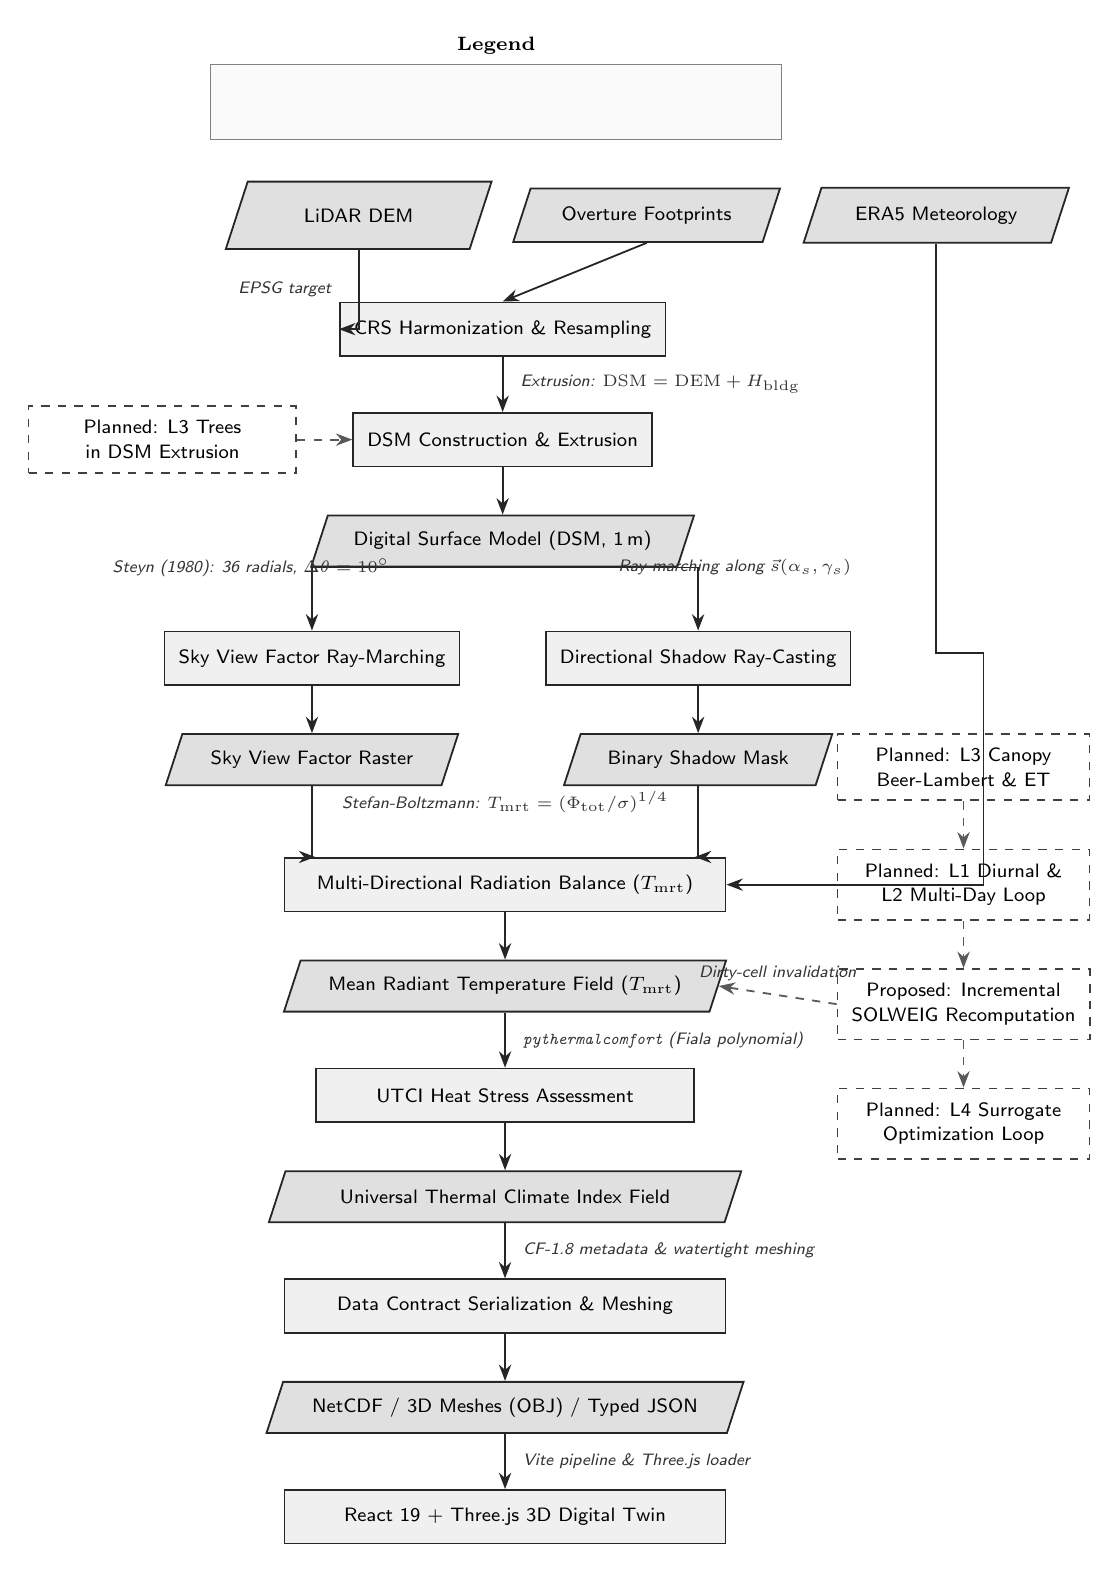
\begin{tikzpicture}[
    >=Stealth,
    node distance=5mm and 6mm,
    % Process Box Style (Rectangle)
    proc/.style={
        rectangle,
        draw=black!85,
        fill=black!6,
        line width=0.65pt,
        minimum width=3.4cm,
        minimum height=0.68cm,
        align=center,
        inner sep=1.8mm,
        font=\sffamily\fontsize{7.5pt}{9pt}\selectfont
    },
    procdash/.style={
        rectangle,
        draw=black!75,
        fill=white,
        dashed,
        line width=0.65pt,
        minimum width=3.4cm,
        minimum height=0.68cm,
        align=center,
        inner sep=1.8mm,
        font=\sffamily\fontsize{7.5pt}{9pt}\selectfont
    },
    % Data Product Style (Parallelogram via trapezium)
    dataprod/.style={
        trapezium,
        trapezium left angle=72,
        trapezium right angle=108,
        draw=black!85,
        fill=black!12,
        line width=0.65pt,
        minimum width=3.4cm,
        minimum height=0.65cm,
        align=center,
        inner sep=1.8mm,
        font=\sffamily\fontsize{7.5pt}{9pt}\selectfont
    },
    dataproddash/.style={
        trapezium,
        trapezium left angle=72,
        trapezium right angle=108,
        draw=black!75,
        fill=white,
        dashed,
        line width=0.65pt,
        minimum width=3.4cm,
        minimum height=0.65cm,
        align=center,
        inner sep=1.8mm,
        font=\sffamily\fontsize{7.5pt}{9pt}\selectfont
    },
    conn/.style={
        ->,
        draw=black!85,
        line width=0.65pt
    },
    conndash/.style={
        ->,
        draw=black!65,
        dashed,
        line width=0.65pt
    },
    eqlabel/.style={
        font=\sffamily\fontsize{6.5pt}{8pt}\itshape,
        text=black!80,
        align=left
    }
]

% =========================================================================
% STAGE 1: RAW INPUTS (PARALLELOGRAMS)
% =========================================================================
\node[dataprod] (d_dem) {LiDAR DEM};
\node[dataprod, right=5mm of d_dem] (d_bldg) {Overture Footprints};
\node[dataprod, right=5mm of d_bldg] (d_met) {ERA5 Meteorology};

% =========================================================================
% STAGE 2: HARMONIZATION & DSM BUILD (RECTANGLES)
% =========================================================================
\node[proc, below=7mm of $(d_dem.south)!0.5!(d_bldg.south)$] (p_crs) {CRS Harmonization \& Resampling};
\node[proc, below=7mm of p_crs] (p_dsm) {DSM Construction \& Extrusion};
\node[dataprod, below=6mm of p_dsm] (d_dsm) {Digital Surface Model (DSM, 1\,m)};

% Optional Planned Tree Integration
\node[procdash, left=7mm of p_dsm] (p_tree) {Planned: L3 Trees\\in DSM Extrusion};

% =========================================================================
% STAGE 3: RADIATIVE TRANSFER SPLIT (SVF & SHADOWS)
% =========================================================================
\node[proc, below left=8mm and 2mm of d_dsm] (p_svf) {Sky View Factor Ray-Marching};
\node[proc, below right=8mm and 2mm of d_dsm] (p_shd) {Directional Shadow Ray-Casting};

\node[dataprod, below=6mm of p_svf] (d_svf) {Sky View Factor Raster};
\node[dataprod, below=6mm of p_shd] (d_shd) {Binary Shadow Mask};

% =========================================================================
% STAGE 4: MEAN RADIANT TEMPERATURE & UTCI
% =========================================================================
\node[proc, below=9mm of $(d_svf.south)!0.5!(d_shd.south)$, minimum width=5.6cm] (p_mrt) {Multi-Directional Radiation Balance ($T_{\mathrm{mrt}}$)};
\node[dataprod, below=6mm of p_mrt] (d_mrt) {Mean Radiant Temperature Field ($T_{\mathrm{mrt}}$)};

\node[proc, below=7mm of d_mrt, minimum width=4.8cm] (p_utci) {UTCI Heat Stress Assessment};
\node[dataprod, below=6mm of p_utci] (d_utci) {Universal Thermal Climate Index Field};

% =========================================================================
% STAGE 5: EXPORTS & DIGITAL TWIN VISUALIZATION
% =========================================================================
\node[proc, below=7mm of d_utci, minimum width=5.6cm] (p_exp) {Data Contract Serialization \& Meshing};
\node[dataprod, below=6mm of p_exp] (d_exp) {NetCDF / 3D Meshes (OBJ) / Typed JSON};
\node[proc, below=7mm of d_exp, minimum width=5.6cm] (p_ui) {React 19 + Three.js 3D Digital Twin};

% =========================================================================
% PLANNED & PROPOSED FEEDBACK / ADVANCED MODULES (RIGHT COLUMN)
% =========================================================================
\node[procdash, right=14mm of p_mrt, minimum width=3.2cm] (p_l1l2) {Planned: L1 Diurnal \&\\L2 Multi-Day Loop};
\node[procdash, above=6mm of p_l1l2, minimum width=3.2cm] (p_canopy) {Planned: L3 Canopy\\Beer-Lambert \& ET};
\node[procdash, below=6mm of p_l1l2, minimum width=3.2cm] (p_inc) {Proposed: Incremental\\SOLWEIG Recomputation};
\node[procdash, below=6mm of p_inc, minimum width=3.2cm] (p_opt) {Planned: L4 Surrogate\\Optimization Loop};

% =========================================================================
% ARROWS & METHOD LABELS (ORTHOGONAL ONLY)
% =========================================================================
% Inputs to CRS
\draw[conn] (d_dem.south) |- (p_crs.west);
\draw[conn] (d_bldg.south) -- (p_crs.north);
\path (d_dem.south) -- node[eqlabel, left=1mm] {EPSG target} (p_crs.west);

% CRS to DSM
\draw[conn] (p_crs.south) -- node[eqlabel, right=1mm] {Extrusion: $\mathrm{DSM} = \mathrm{DEM} + H_{\mathrm{bldg}}$} (p_dsm.north);
\draw[conndash] (p_tree.east) -- (p_dsm.west);
\draw[conn] (p_dsm.south) -- (d_dsm.north);

% DSM to SVF and Shadows
\draw[conn] (d_dsm.south) -| node[eqlabel, pos=0.25, left=1mm] {Steyn (1980): 36 radials, $\Delta \theta = 10^\circ$} (p_svf.north);
\draw[conn] (d_dsm.south) -| node[eqlabel, pos=0.25, right=1mm] {Ray-marching along $\vec{s}(\alpha_s, \gamma_s)$} (p_shd.north);

\draw[conn] (p_svf.south) -- (d_svf.north);
\draw[conn] (p_shd.south) -- (d_shd.north);

% SVF, Shadows, and ERA5 to Tmrt
\draw[conn] (d_svf.south) |- ($(p_mrt.north west)+(4mm,0)$);
\draw[conn] (d_shd.south) |- ($(p_mrt.north east)+(-4mm,0)$);
\draw[conn] (d_met.south) |- ++(6mm,-5.2cm) |- (p_mrt.east);
\path ($(d_svf.south)!0.5!(d_shd.south)$) -- node[eqlabel, yshift=2.5mm] {Stefan-Boltzmann: $T_{\mathrm{mrt}} = (\Phi_{\mathrm{tot}} / \sigma)^{1/4}$} (p_mrt.north);

\draw[conn] (p_mrt.south) -- (d_mrt.north);

% Tmrt to UTCI
\draw[conn] (d_mrt.south) -- node[eqlabel, right=1mm] {\texttt{pythermalcomfort} (Fiala polynomial)} (p_utci.north);
\draw[conn] (p_utci.south) -- (d_utci.north);

% UTCI to Export
\draw[conn] (d_utci.south) -- node[eqlabel, right=1mm] {CF-1.8 metadata \& watertight meshing} (p_exp.north);
\draw[conn] (p_exp.south) -- (d_exp.north);

% Export to UI
\draw[conn] (d_exp.south) -- node[eqlabel, right=1mm] {Vite pipeline \& Three.js loader} (p_ui.north);

% Planned connections
\draw[conndash] (p_canopy.south) -- (p_l1l2.north);
\draw[conndash] (p_l1l2.south) -- (p_inc.north);
\draw[conndash] (p_inc.south) -- (p_opt.north);
\draw[conndash] (p_inc.west) -- node[eqlabel, above=0.5mm] {Dirty-cell invalidation} (d_mrt.east);

% =========================================================================
% LEGEND (TOP LEFT)
% =========================================================================
\node[proc, minimum width=1.5cm, minimum height=0.45cm, font=\fontsize{6.5pt}{7.5pt}\selectfont] at ($(d_dem.north west)+(-5mm, 10mm)$) (l_proc) {Process};
\node[dataprod, minimum width=1.5cm, minimum height=0.45cm, font=\fontsize{6.5pt}{7.5pt}\selectfont, right=4mm of l_proc] (l_data) {Data Product};
\node[procdash, minimum width=1.5cm, minimum height=0.45cm, font=\fontsize{6.5pt}{7.5pt}\selectfont, right=4mm of l_data] (l_dash) {Planned/Proposed};

\node[draw=black!50, fill=black!2, inner sep=1.8mm, fit=(l_proc) (l_data) (l_dash), label={[font=\fontsize{7pt}{8pt}\bfseries]north:Legend}] {};

\end{tikzpicture}
\end{document}
